    \documentclass[dvipsnames]{beamer}
    \usetheme{Madrid}
    \usefonttheme{professionalfonts}
    \usepackage{
        amsmath,
        amssymb,
        fouriernc, % fourier font w/ new century book
        fancyhdr, % page styling
        lastpage, % footer fanciness
        hyperref, % various links
        setspace, % line spacing
        amsthm, % newtheorem and proof environment
        mathtools, % \Aboxed for boxing inside aligns, among others
        float, % Allow [H] figure env alignment
        enumerate, % Allow custom enumerate numbering
        graphicx, % allow includegraphics with more filetypes
        wasysym, % \smiley!
        upgreek, % \upmu for \mum macro
        listings, % writing TrueType fonts and including code prettily
        tikz, % drawing things
        booktabs, % \bottomrule instead of hline apparently
        cancel % can cancel things out!
    }
    \usepackage[
        labelfont=bf, % caption names are labeled in bold
        font=scriptsize % smaller font for captions
    ]{caption}
    \usepackage[font=scriptsize]{subcaption} % subfigures

    \newcommand*{\scinot}[2]{#1\times10^{#2}}
    \newcommand*{\dotp}[2]{\left<#1\,\middle|\,#2\right>}
    \newcommand*{\rd}[2]{\frac{\mathrm{d}#1}{\mathrm{d}#2}}
    \newcommand*{\pd}[2]{\frac{\partial#1}{\partial#2}}
    \newcommand*{\rtd}[2]{\frac{\mathrm{d}^2#1}{\mathrm{d}#2^2}}
    \newcommand*{\ptd}[2]{\frac{\partial^2 #1}{\partial#2^2}}
    \newcommand*{\md}[2]{\frac{\mathrm{D}#1}{\mathrm{D}#2}}
    \newcommand*{\pvec}[1]{\vec{#1}^{\,\prime}}
    \newcommand*{\svec}[1]{\vec{#1}\;\!}
    \newcommand*{\bm}[1]{\boldsymbol{\mathbf{#1}}}
    \newcommand*{\ang}[0]{\;\text{\AA}}
    \newcommand*{\mum}[0]{\;\upmu \mathrm{m}}
    \newcommand*{\at}[1]{\left.#1\right|}

    \let\Re\undefined
    \let\Im\undefined
    \DeclareMathOperator{\Res}{Res}
    \DeclareMathOperator{\Re}{Re}
    \DeclareMathOperator{\Im}{Im}
    \DeclareMathOperator{\Log}{Log}
    \DeclareMathOperator{\Arg}{Arg}
    \DeclareMathOperator{\Tr}{Tr}
    \DeclareMathOperator{\E}{E}
    \DeclareMathOperator{\Var}{Var}
    \DeclareMathOperator*{\argmin}{argmin}
    \DeclareMathOperator*{\argmax}{argmax}
    \DeclareMathOperator{\sgn}{sgn}
    \DeclareMathOperator{\diag}{diag\;}

    \DeclarePairedDelimiter\bra{\langle}{\rvert}
    \DeclarePairedDelimiter\ket{\lvert}{\rangle}
    \DeclarePairedDelimiter\abs{\lvert}{\rvert}
    \DeclarePairedDelimiter\ev{\langle}{\rangle}
    \DeclarePairedDelimiter\p{\lparen}{\rparen}
    \DeclarePairedDelimiter\s{\lbrack}{\rbrack}
    \DeclarePairedDelimiter\z{\lbrace}{\rbrace}

    % \everymath{\displaystyle} % biggify limits of inline sums and integrals
    \tikzstyle{circ} % usage: \node[circ, placement] (label) {text};
        = [draw, circle, fill=white, node distance=3cm, minimum height=2em]
    \definecolor{commentgreen}{rgb}{0,0.6,0}
    \lstset{
        basicstyle=\ttfamily\footnotesize,
        frame=single,
        numbers=left,
        showstringspaces=false,
        keywordstyle=\color{blue},
        stringstyle=\color{purple},
        commentstyle=\color{commentgreen},
        morecomment=[l][\color{magenta}]{\#}
    }

\begin{document}

\begin{frame}
    \frametitle{Linear}

    \begin{figure}[t]
        \centering
        \includegraphics[width=0.7\textwidth]{../sims/2d_3_final/snapshots_lin_0/fluxes.png}
        \caption{Linear simulation.}
    \end{figure}
\end{frame}

\begin{frame}
    \frametitle{New Plotting for Nonlinear}

    \begin{figure}[t]
        \centering
        \includegraphics[width=0.7\textwidth]{../sims/2d_3_final/snapshots_nl_3/fluxes.png}
        \caption{Nonlinear simulation, new plotting methodology. Feedback?}
    \end{figure}
\end{frame}

\begin{frame}
    \frametitle{Reflection?}

    Get exact solution, up to viscous dissipation. Plot $\delta u_z =
    \frac{u_{z,sim} - u_{z, anal}}{\abs*{u_{z, anal}}}$, ``fractional
    deviation'' between driving zone and critical layer. Compute $\mathrm{RMS} =
    \sqrt{\ev*{\delta u_z^2}}$.
    \begin{figure}[t]
        \centering
        \includegraphics[width=0.7\textwidth]{../sims/2d_3_final/snapshots_lin_1/p_074.png}
        \caption{Linear simulation with same viscosity as nonlinear. Green is
        viscosity-free envelope, orange analytical.}
    \end{figure}
\end{frame}

\begin{frame}
    \frametitle{Reflection (nl4)}

    Get exact solution, up to viscous dissipation. Plot $\delta u_z =
    \frac{u_{z,sim} - u_{z, anal}}{\abs*{u_{z, anal}}}$, ``fractional
    deviation'' between driving zone and critical layer. Compute $\mathrm{RMS} =
    \sqrt{\ev*{\delta u_z^2}}$.
    \begin{figure}[t]
        \centering
        \includegraphics[width=0.7\textwidth]{../sims/2d_3_final/snapshots_nl_4/p_074.png}
        \caption{Nonlinear simulation. Green is viscosity-free envelope, orange
        analytical.}
    \end{figure}
\end{frame}

\begin{frame}
    \frametitle{Reflection?}

    \begin{table}[t]
        \centering
        \begin{tabular}{l|l l }
            Name & RMS & Notes\\
            lin0 & 0.077 & Almost-no visc\\
            lin1 & 0.067 & Same visc as nl4\\
            nl1 (low) & 0.132 & half-res nl1, higher visc\\
            nl1 & 0.120 & $0.7\nu$\\
            nl2 & 0.213 & $0.4\nu$\\
            nl3 & 0.179 & $0.4\nu$ (double A)\\
            nl4 & 0.269 & $0.3\nu$\\
            nl5 & 0.207 & $0.3\nu$ (double $k_z$)\\
            nl6 & 0.246 & $0.2\nu$\\
            nl7 & 0.358 & $0.1\nu$
        \end{tabular}
        \caption{Table of RMS values.}
    \end{table}
\end{frame}

\begin{frame}
    \frametitle{Reflection (nl6)}

    Get exact solution, up to viscous dissipation. Plot $\delta u_z =
    \frac{u_{z,sim} - u_{z, anal}}{\abs*{u_{z, anal}}}$, ``fractional
    deviation'' between driving zone and critical layer. Compute $\mathrm{RMS} =
    \sqrt{\ev*{\delta u_z^2}}$.
    \begin{figure}[t]
        \centering
        \includegraphics[width=0.7\textwidth]{../sims/2d_3_final/snapshots_nl_6/p_074.png}
        \caption{Nonlinear simulation. Green is viscosity-free envelope, orange
        analytical.}
    \end{figure}
\end{frame}

\begin{frame}
    \frametitle{Reflection (nl7)}

    Get exact solution, up to viscous dissipation. Plot $\delta u_z =
    \frac{u_{z,sim} - u_{z, anal}}{\abs*{u_{z, anal}}}$, ``fractional
    deviation'' between driving zone and critical layer. Compute $\mathrm{RMS} =
    \sqrt{\ev*{\delta u_z^2}}$.
    \begin{figure}[t]
        \centering
        \includegraphics[width=0.7\textwidth]{../sims/2d_3_final/snapshots_nl_7/p_074.png}
        \caption{Nonlinear simulation. Green is viscosity-free envelope, orange
        analytical.}
    \end{figure}
\end{frame}

\begin{frame}
    \frametitle{Reflection (nl3)}

    Get exact solution, up to viscous dissipation. Plot $\delta u_z =
    \frac{u_{z,sim} - u_{z, anal}}{\abs*{u_{z, anal}}}$, ``fractional
    deviation'' between driving zone and critical layer. Compute $\mathrm{RMS} =
    \sqrt{\ev*{\delta u_z^2}}$.
    \begin{figure}[t]
        \centering
        \includegraphics[width=0.7\textwidth]{../sims/2d_3_final/snapshots_nl_3/p_058.png}
        \caption{Nonlinear simulation. Green is viscosity-free envelope, orange
        analytical.}
    \end{figure}
\end{frame}

\begin{frame}
    \frametitle{Reflection (nl5)}

    Get exact solution, up to viscous dissipation. Plot $\delta u_z =
    \frac{u_{z,sim} - u_{z, anal}}{\abs*{u_{z, anal}}}$, ``fractional
    deviation'' between driving zone and critical layer. Compute $\mathrm{RMS} =
    \sqrt{\ev*{\delta u_z^2}}$.
    \begin{figure}[t]
        \centering
        \includegraphics[width=0.7\textwidth]{../sims/2d_3_final/snapshots_nl_5/p_074.png}
        \caption{Nonlinear simulation. Green is viscosity-free envelope, orange
        analytical.}
    \end{figure}
\end{frame}

\end{document}

